% Chapter 3: Supervised Learning
\chapter{Supervised Learning}

\section{Problem Formulation}
The prediction task is formulated as binary classification:
\begin{itemize}
    \item \textbf{Class 1:} Fire detected at location
    \item \textbf{Class 0:} No fire detected at location
\end{itemize}

The dataset maintains an approximate 60\%/40\% class distribution (no fire/fire) after preprocessing, with stratified train/test splits (80\%/20\%) preserving this ratio.

\section{Feature Engineering}

Starting from the merged dataset with 42+ raw features, we applied a systematic pipeline to extract, select, and scale features for optimal model performance.

\subsection{Feature Extraction}
We created 22 new features based on domain knowledge:

\textbf{Climate-based features (9):}
\begin{itemize}
    \item \texttt{annual\_temp\_range}, \texttt{avg\_tmax}, \texttt{avg\_tmin}, \texttt{diurnal\_temp\_range}
    \item \texttt{total\_annual\_precip}, \texttt{summer\_precip\_ratio}, \texttt{precip\_variability}
    \item \texttt{summer\_heat\_index}, \texttt{drought\_index} = $\frac{\text{tmax\_summer}}{\text{prec\_summer} + 1}$
\end{itemize}

\textbf{Topography-based features (4):}
\begin{itemize}
    \item \texttt{terrain\_complexity} = slope $\times$ roughness
    \item \texttt{elevation\_slope\_interaction} = elevation $\times$ slope
    \item \texttt{aspect\_cardinal}: Aspect converted to cardinal directions (N/E/S/W)
    \item \texttt{is\_south\_facing}: Binary indicator for south-facing slopes
\end{itemize}

\textbf{Soil-based features (6):}
\begin{itemize}
    \item \texttt{sand\_clay\_ratio}, \texttt{fine\_fraction} (silt + clay)
    \item \texttt{fertility\_index}, \texttt{moisture\_retention}
    \item \texttt{ph\_carbon\_interaction}, \texttt{nutrient\_availability}
\end{itemize}

\textbf{Spatial features (3):}
\begin{itemize}
    \item \texttt{country}: Binary indicator (Algeria/Tunisia based on longitude)
    \item \texttt{coastal\_proximity} = $37 - \text{latitude}$
    \item \texttt{lat\_long\_interaction} = latitude $\times$ longitude
\end{itemize}

\subsection{Feature Selection}
A multi-step selection process reduced features from 60+ to 20:

\textbf{Step 1: Multicollinearity Removal}
\begin{itemize}
    \item Threshold: Feature-to-feature correlation $> 0.90$
    \item For correlated pairs, kept the feature with higher target correlation
\end{itemize}

\textbf{Step 2: Target Correlation Selection}
\begin{itemize}
    \item Selected top 30 features by absolute correlation with target variable
\end{itemize}

\textbf{Step 3: Composite Scoring}
Applied four methods and combined normalized scores:
\begin{enumerate}
    \item ANOVA F-test scores
    \item Mutual Information scores
    \item Random Forest feature importance
    \item Target correlation
\end{enumerate}

\begin{equation}
    \text{Composite Score} = \frac{1}{4}\sum_{i=1}^{4} \text{Normalized}(\text{Method}_i)
\end{equation}

Final selection: Top 20 features by composite score.

\begin{figure}[H]
    \centering
    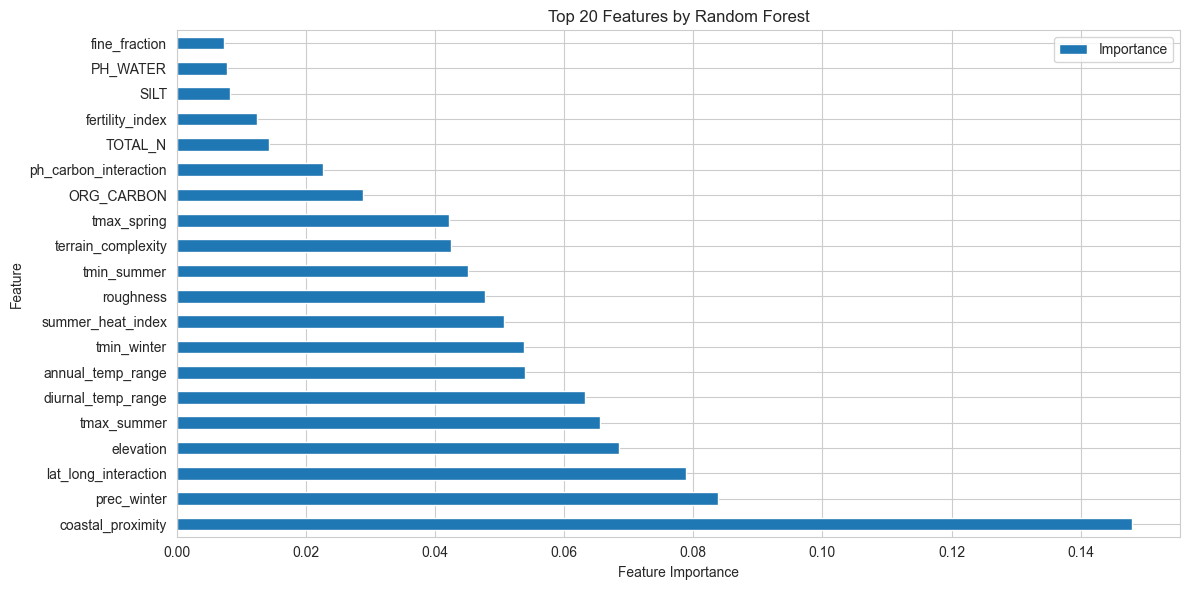
\includegraphics[width=1.0\textwidth]{ressources/chapter3/feature_engineering_supervised/top20_features_by_random_forest.png}
    \caption{Top 20 features ranked by Random Forest feature importance. Geographic and climate-related features dominate, with coastal proximity and drought index showing highest predictive power.}
    \label{fig:top20_features}
\end{figure}

\subsection{Feature Scaling}
StandardScaler (z-score normalization) applied to all 20 selected features:
\begin{equation}
    z = \frac{x - \mu}{\sigma}
\end{equation}

\begin{table}[H]
\centering
\caption{Feature Statistics Before and After Scaling (Sample of 5 Features)}
\label{tab:scaling_comparison}
\begin{tabular}{|l|c|c|c|c|c|c|c|c|}
\hline
\multirow{2}{*}{\textbf{Feature}} & \multicolumn{4}{c|}{\textbf{Before Scaling}} & \multicolumn{4}{c|}{\textbf{After Scaling}} \\
\cline{2-9}
 & Mean & Std & Min & Max & Mean & Std & Min & Max \\
\hline
coastal\_proximity & 2.15 & 1.42 & -0.89 & 6.12 & 0.00 & 1.00 & -2.14 & 2.79 \\
drought\_index & 8.34 & 5.67 & 0.45 & 32.18 & 0.00 & 1.00 & -1.39 & 4.20 \\
elevation & 456.2 & 312.8 & 12 & 1892 & 0.00 & 1.00 & -1.42 & 4.59 \\
prec\_winter & 67.4 & 42.1 & 8.2 & 215.6 & 0.00 & 1.00 & -1.41 & 3.52 \\
tmax\_summer & 35.2 & 4.8 & 24.1 & 45.6 & 0.00 & 1.00 & -2.31 & 2.17 \\
\hline
\end{tabular}
\end{table}

\textbf{Note:} Scaling is essential for KNN (distance-based) but applied uniformly for consistency. Tree-based methods are invariant to monotonic transformations.

\subsection{Feature Engineering Summary}

\begin{table}[H]
\centering
\caption{Feature Engineering Pipeline Statistics}
\label{tab:fe_summary}
\begin{tabular}{|l|c|c|}
\hline
\textbf{Stage} & \textbf{Features} & \textbf{Description} \\
\hline
Original dataset & 41 & Raw merged features \\
After feature extraction & 63 & +22 domain-specific features \\
After one-hot encoding & 65 & TEXTURE\_SOTER encoded \\
After multicollinearity removal & 47 & Removed $r > 0.90$ pairs \\
After target correlation & 30 & Top 30 by $|r|$ with target \\
Final selection & 20 & Top 20 by composite score \\
\hline
\textbf{Reduction} & \textbf{51\%} & 41 $\rightarrow$ 20 features \\
\hline
\end{tabular}
\end{table}

\section{K-Nearest Neighbors (KNN)}

\subsection{Hyperparameter Tuning}
Optimal $k$ selected by evaluating $k \in \{3, 5, 7, 9, 11\}$ on the test set using Euclidean distance, with maximum F1-score as the selection criterion.

\begin{figure}[H]
    \centering
    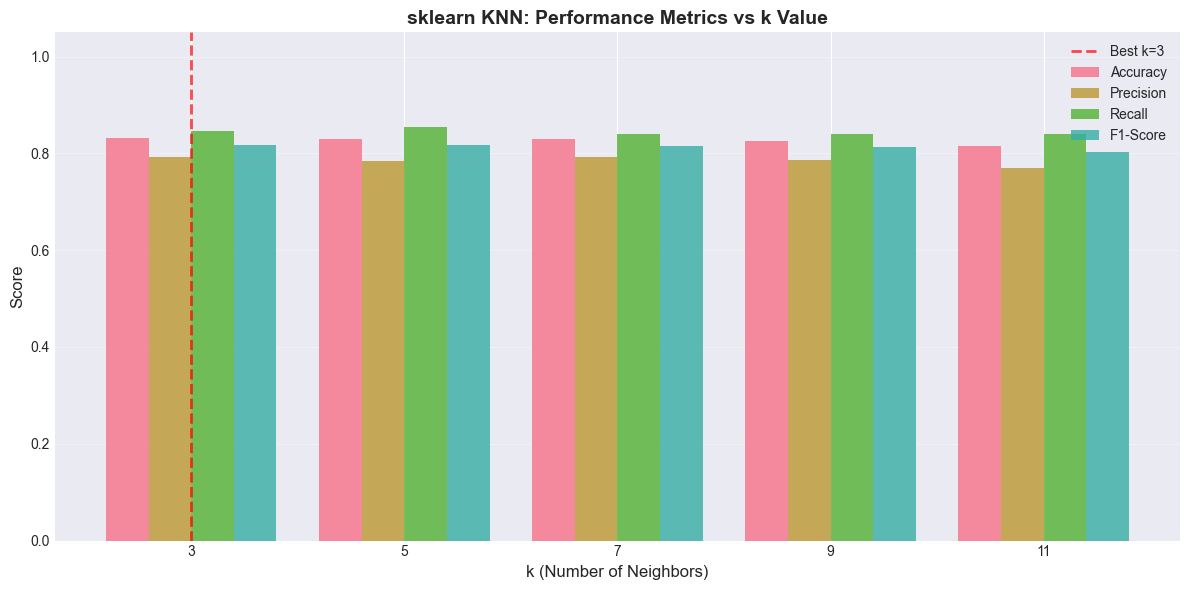
\includegraphics[width=1.0\textwidth]{ressources/chapter3/KNN/metrics_vs_kvalue.png}
    \caption{Performance metrics (accuracy, precision, recall, F1-score) for different $k$ values. The best performance is achieved at $k=3$ with the highest F1-score.}
    \label{fig:knn_cv}
\end{figure}

\begin{table}[H]
\centering
\caption{sklearn KNN Performance for Different $k$ Values}
\label{tab:knn_k_tuning}
\begin{tabular}{|c|c|c|c|c|}
\hline
\textbf{k} & \textbf{Accuracy} & \textbf{Precision} & \textbf{Recall} & \textbf{F1-Score} \\
\hline
3 & 0.8059 & 0.7769 & 0.8584 & \textbf{0.8156} \\
5 & 0.7991 & 0.7764 & 0.8402 & 0.8070 \\
7 & 0.7823 & 0.7531 & 0.8402 & 0.7942 \\
9 & 0.7854 & 0.7558 & 0.8432 & 0.7971 \\
11 & 0.7854 & 0.7608 & 0.8326 & 0.7951 \\
\hline
\end{tabular}
\end{table}

\subsection{Dataset Comparison}
We compared custom KNN performance on original (41 features) vs. engineered (20 features) datasets:

\begin{figure}[H]
    \centering
    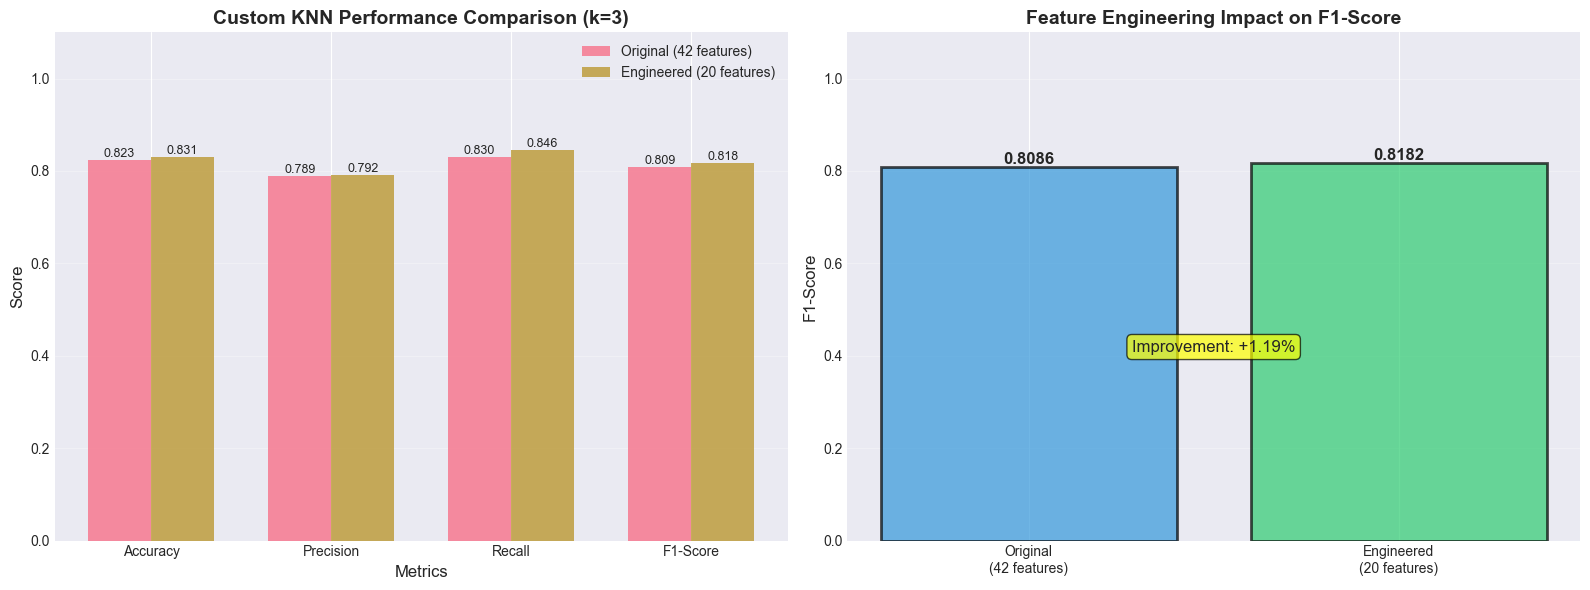
\includegraphics[width=1.0\textwidth]{ressources/chapter3/KNN/original_vs_engineered_comparison.png}
    \caption{Custom KNN performance comparison between original dataset (41 features) and engineered dataset (20 features). Feature engineering improves F1-score while reducing dimensionality.}
    \label{fig:knn_dataset_comparison}
\end{figure}

\begin{table}[H]
\centering
\caption{Custom KNN Performance Comparison ($k=3$)}
\label{tab:knn_comparison}
\begin{tabular}{|l|c|c|c|c|c|}
\hline
\textbf{Dataset} & \textbf{Features} & \textbf{Accuracy} & \textbf{Precision} & \textbf{Recall} & \textbf{F1} \\
\hline
Original & 41 & 0.7960 & 0.7675 & 0.8493 & 0.8064 \\
Engineered & 20 & 0.8059 & 0.7769 & 0.8584 & 0.8156 \\
\hline
\end{tabular}
\end{table}

\textbf{Finding:} Feature engineering improved F1-score by 1.1\% while reducing dimensionality by 51\%, demonstrating effective feature selection.

\begin{figure}[H]
    \centering
    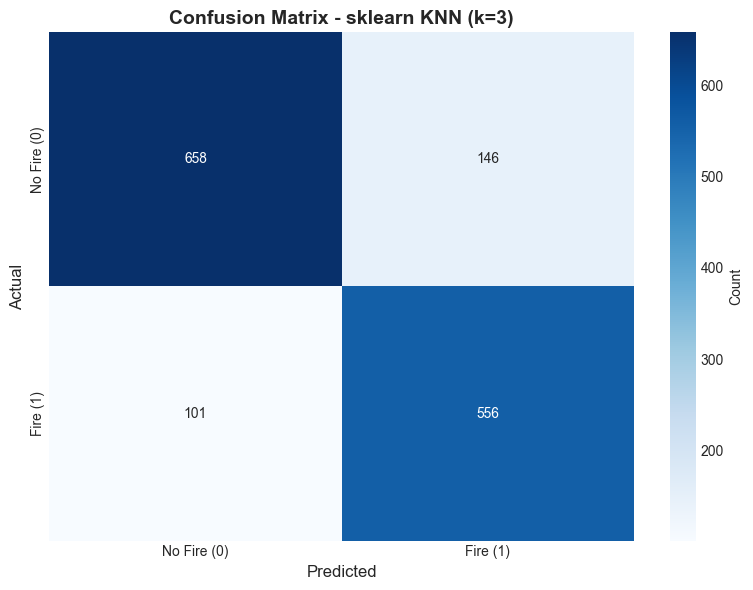
\includegraphics[width=0.8\textwidth]{ressources/chapter3/KNN/confusion_matrix.png}
    \caption{Confusion matrix for the best KNN model ($k=3$) showing the distribution of true positives, false positives, true negatives, and false negatives.}
    \label{fig:knn_confusion}
\end{figure}

\section{Decision Tree}

\subsection{Hyperparameter Tuning}
Bayesian Optimization with Gaussian Processes was used to find optimal parameters:
\begin{itemize}
    \item \texttt{max\_depth} $\in [2, 30]$
    \item \texttt{min\_samples\_split} $\in [2, 50]$
    \item \texttt{min\_samples\_leaf} $\in [1, 20]$
    \item Objective: Maximize F1-score via 5-fold stratified cross-validation
    \item Total evaluations: 40 (10 random initial + 30 Bayesian)
\end{itemize}

\textbf{Best parameters found:} max\_depth = 30, min\_samples\_split = 2, min\_samples\_leaf = 1.

\begin{figure}[H]
    \centering
    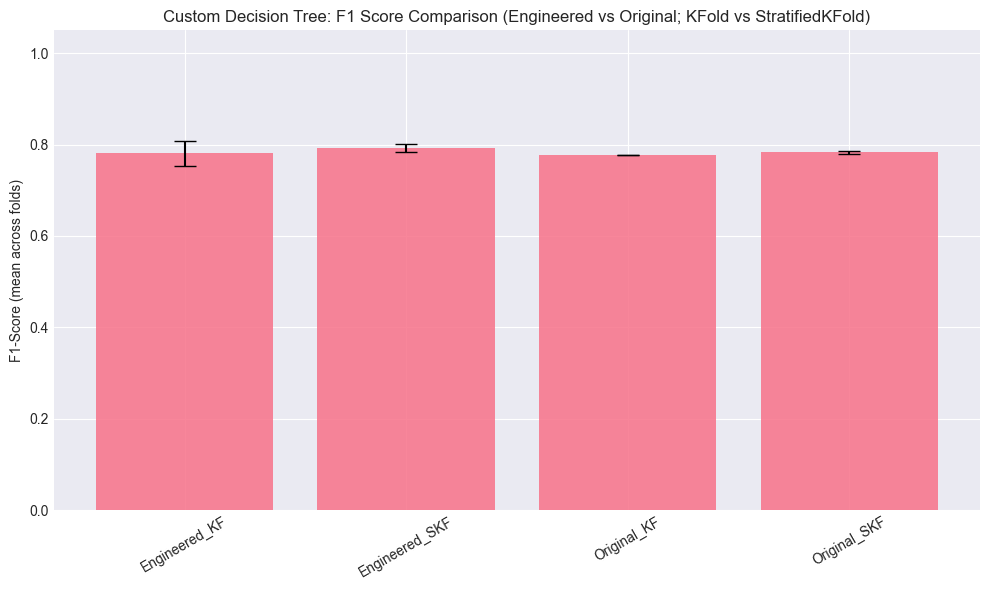
\includegraphics[width=1.0\textwidth]{ressources/chapter3/decision_tree/f1score_comparison.png}
    \caption{F1-score comparison across different dataset and cross-validation configurations. Stratified K-Fold consistently outperforms regular K-Fold, and engineered features show improved performance.}
    \label{fig:dt_f1_comparison}
\end{figure}

\subsection{Implementation Comparison}
We compared sklearn's DecisionTreeClassifier with a custom implementation using the optimal parameters:

\begin{figure}[H]
    \centering
    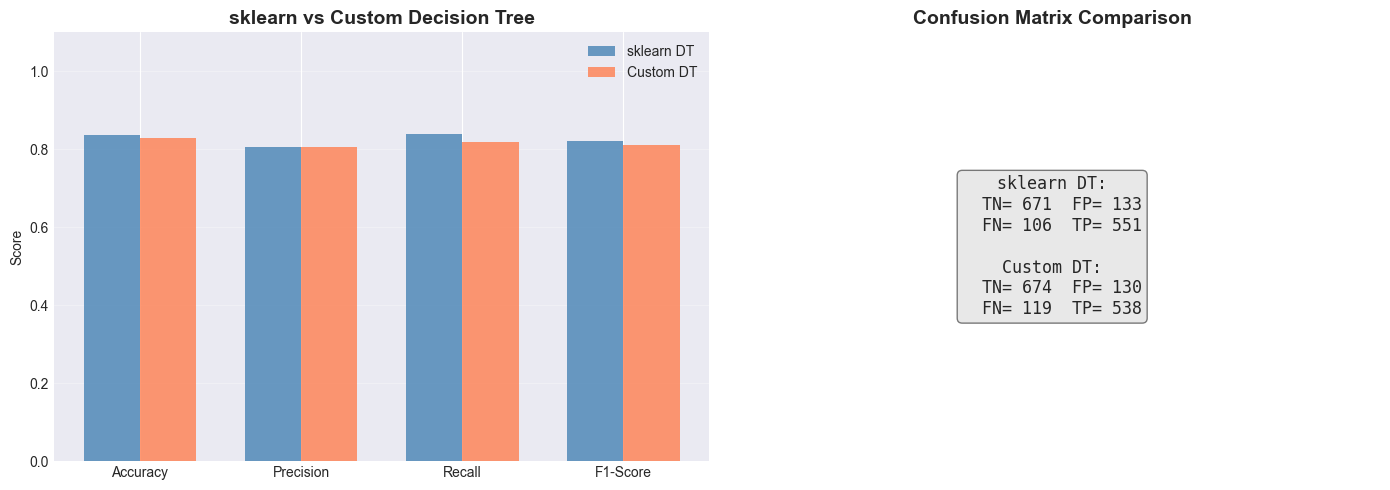
\includegraphics[width=1.0\textwidth]{ressources/chapter3/decision_tree/sk_vs_custom.png}
    \caption{Performance comparison between sklearn and custom Decision Tree implementations. Both achieve comparable results, validating the custom implementation.}
    \label{fig:dt_sk_vs_custom}
\end{figure}

\begin{table}[H]
\centering
\caption{sklearn vs Custom Decision Tree Performance}
\label{tab:dt_comparison}
\begin{tabular}{|l|c|c|c|c|}
\hline
\textbf{Implementation} & \textbf{Accuracy} & \textbf{Precision} & \textbf{Recall} & \textbf{F1} \\
\hline
sklearn DT & 0.7953 & 0.7756 & 0.8311 & 0.8024 \\
Custom DT & 0.7991 & 0.7903 & 0.8143 & 0.8021 \\
\hline
\end{tabular}
\end{table}

\subsection{Cross-Validation Analysis}
We evaluated both KFold (no stratification) and StratifiedKFold on engineered vs. original datasets, confirming that stratification maintains consistent class ratios across folds.

\begin{figure}[H]
    \centering
    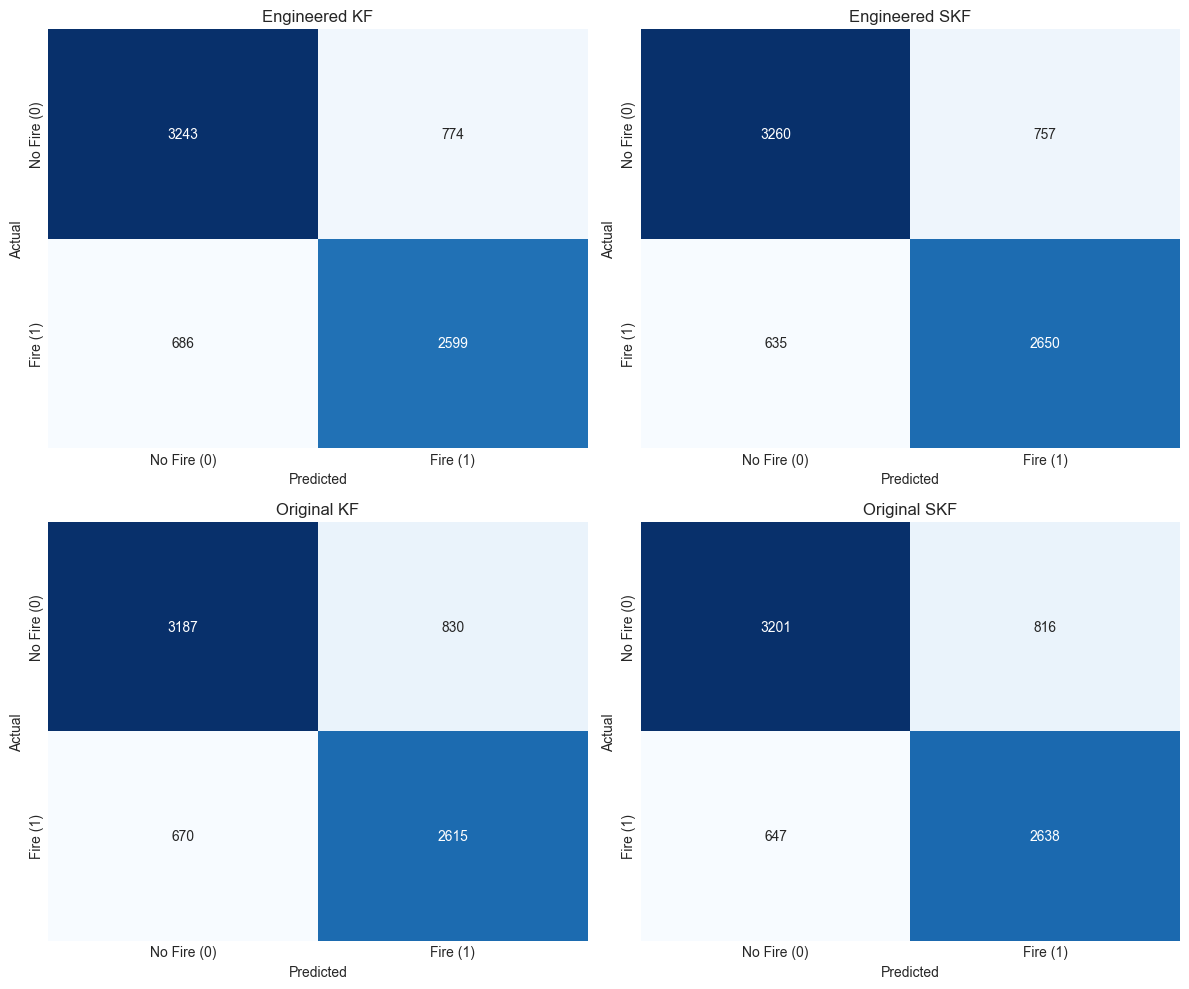
\includegraphics[width=1.0\textwidth]{ressources/chapter3/decision_tree/confusion_matrices.png}
    \caption{Confusion matrices for Decision Tree models across different configurations: Engineered vs Original datasets with KFold and StratifiedKFold cross-validation.}
    \label{fig:dt_confusion}
\end{figure}

\section{Random Forest}

\subsection{Hyperparameter Tuning}
Bayesian Optimization was applied with the following search space:
\begin{itemize}
    \item \texttt{n\_estimators} $\in [10, 200]$
    \item \texttt{max\_depth} $\in [3, 30]$
    \item \texttt{min\_samples\_split} $\in [2, 20]$
    \item \texttt{min\_samples\_leaf} $\in [1, 10]$
    \item \texttt{max\_features}: $\sqrt{n}$
    \item Total evaluations: 40 (10 random initial + 30 Bayesian)
\end{itemize}

\subsection{Implementation Comparison}
Both sklearn's RandomForestClassifier and a custom implementation were evaluated:

\begin{figure}[H]
    \centering
    
\includegraphics[width=1.0\textwidth]{ressources/chapter3/random_forest/sk_vs_custom.png}
    \caption{Performance comparison between sklearn and custom Random Forest implementations across all metrics. Both implementations achieve comparable results.}
    \label{fig:rf_sk_vs_custom}
\end{figure}

\begin{table}[H]
\centering
\caption{sklearn vs Custom Random Forest Performance}
\label{tab:rf_comparison}
\begin{tabular}{|l|c|c|c|c|c|}
\hline
\textbf{Implementation} & \textbf{Accuracy} & \textbf{Precision} & \textbf{Recall} & \textbf{F1} & \textbf{AUC} \\
\hline
sklearn RF & 0.8432 & 0.8235 & 0.8737 & 0.8479 & 0.9062 \\
Custom RF & 0.8105 & 0.7906 & 0.8447 & 0.8168 & 0.8982 \\
\hline
\end{tabular}
\end{table}

\begin{figure}[H]
    \centering
    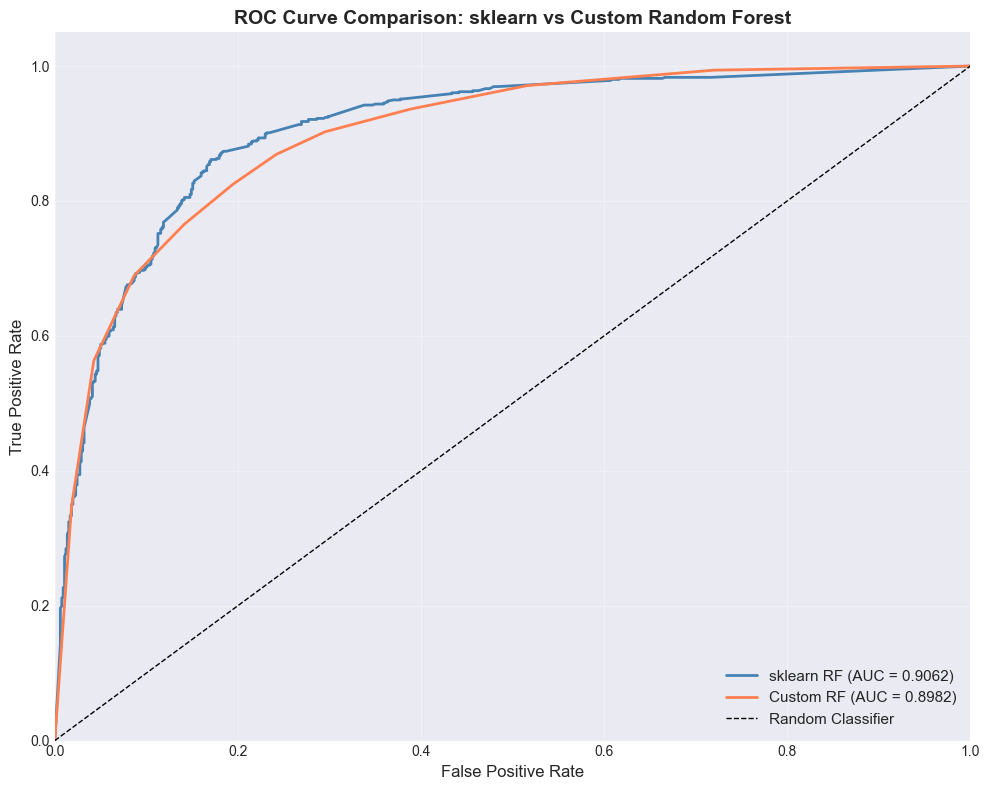
\includegraphics[width=1.0\textwidth]{ressources/chapter3/random_forest/ROC_curve.png}
    \caption{ROC curve comparison between sklearn and custom Random Forest implementations. Both models achieve high AUC scores, indicating excellent discrimination ability.}
    \label{fig:rf_roc}
\end{figure}

\begin{figure}[H]
    \centering
    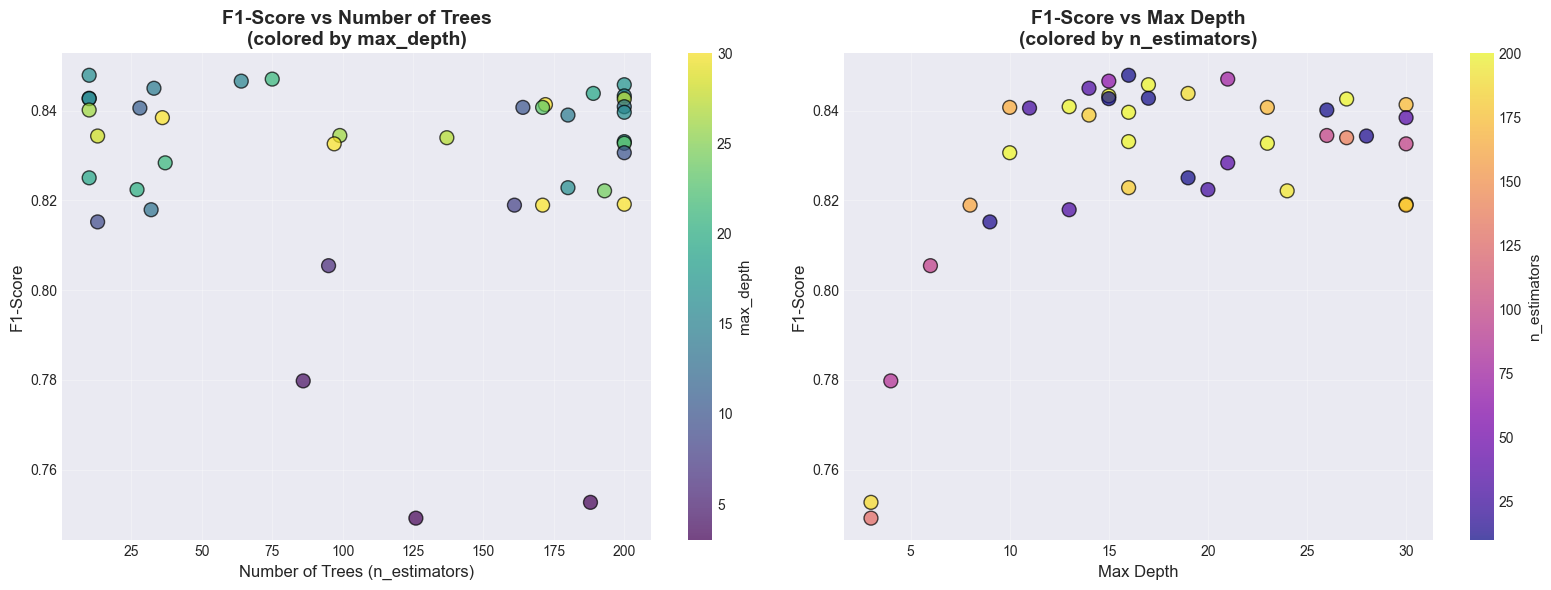
\includegraphics[width=1.0\textwidth]{ressources/chapter3/random_forest/f1_score.png}
    \caption{F1-score comparison between sklearn and custom Random Forest implementations across different configurations.}
    \label{fig:rf_f1_score}
\end{figure}

\begin{figure}[H]
    \centering
    
\includegraphics[width=1.0\textwidth]{ressources/chapter3/random_forest/confusion_matrices.png}
    \caption{Confusion matrices for Random Forest models showing classification performance for sklearn and custom implementations.}
    \label{fig:rf_confusion}
\end{figure}

\subsection{Feature Importance}
Feature importance was computed using Gini importance (sklearn) and feature selection frequency (custom):

\begin{figure}[H]
    \centering
    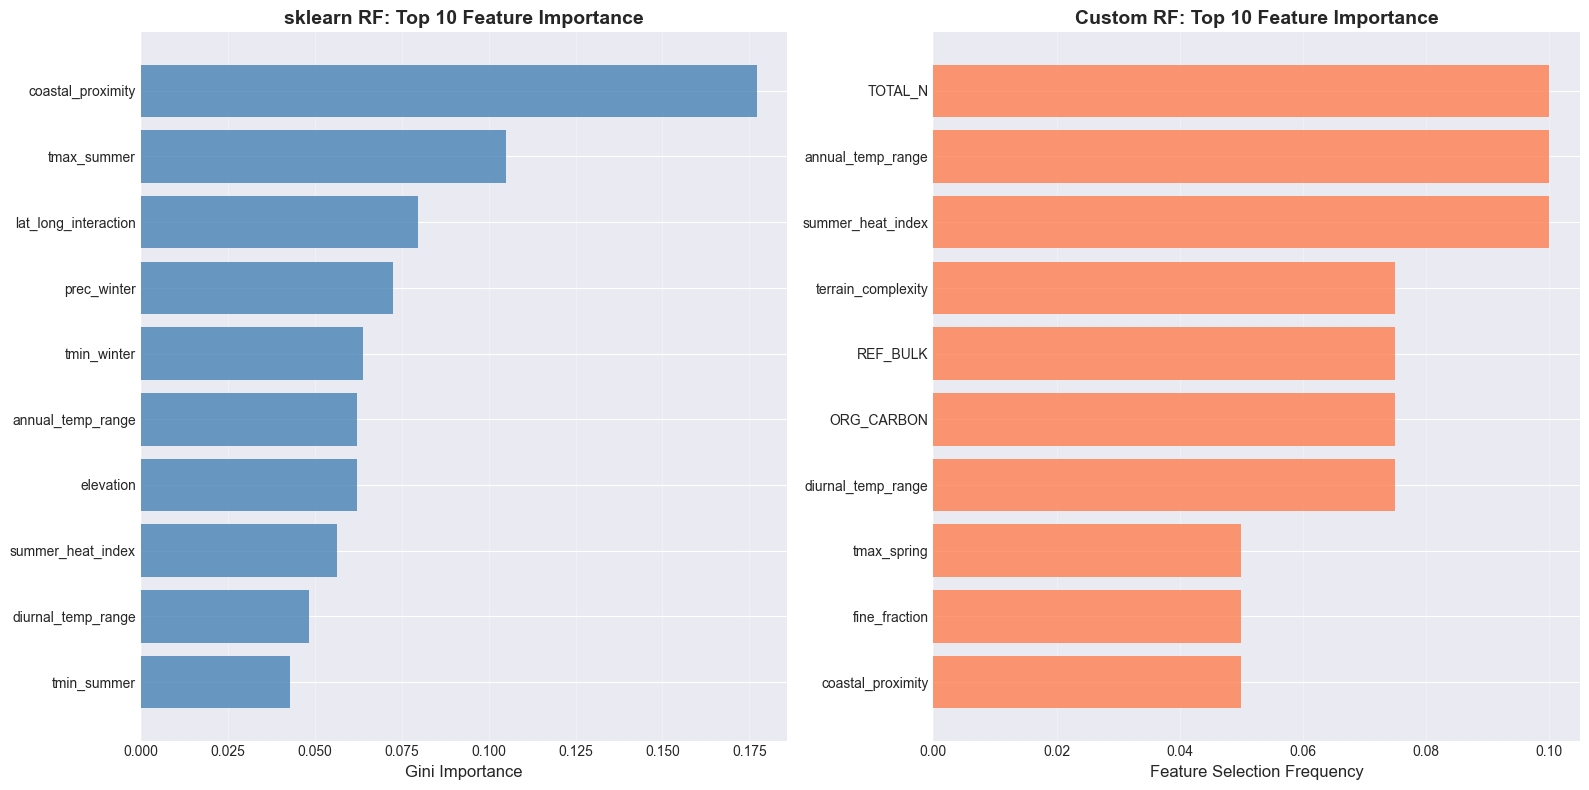
\includegraphics[width=1.0\textwidth]{ressources/chapter3/random_forest/top10_features_importance.png}
    \caption{Top 10 feature importance comparison: sklearn Gini importance vs custom frequency-based importance. Geographic and climate features dominate both rankings.}
    \label{fig:rf_importance}
\end{figure}

\begin{table}[H]
\centering
\caption{Top 10 Features by sklearn Gini Importance}
\label{tab:rf_importance}
\begin{tabular}{|c|l|c|l|}
\hline
\textbf{Rank} & \textbf{Feature} & \textbf{Importance} & \textbf{Interpretation} \\
\hline
1 & coastal\_proximity & 0.1771 & Coastal Mediterranean fire concentration \\
2 & tmax\_summer & 0.1051 & Peak heat conditions \\
3 & lat\_long\_interaction & 0.0796 & Regional geographic patterns \\
4 & prec\_winter & 0.0726 & Antecedent moisture conditions \\
5 & tmin\_winter & 0.0639 & Winter temperature influence \\
6 & annual\_temp\_range & 0.0622 & Temperature variability \\
7 & elevation & 0.0620 & Topographic influence on fires \\
8 & summer\_heat\_index & 0.0564 & Combined heat-moisture stress \\
9 & diurnal\_temp\_range & 0.0485 & Daily temperature swing \\
10 & tmin\_summer & 0.0428 & Summer night temperatures \\
\hline
\end{tabular}
\end{table}

\section{Model Comparison}

\begin{table}[H]
\centering
\caption{Supervised Learning Model Comparison (Engineered Dataset, 20 Features)}
\label{tab:model_comparison}
\begin{tabular}{|l|c|c|c|c|c|}
\hline
\textbf{Model} & \textbf{Accuracy} & \textbf{Precision} & \textbf{Recall} & \textbf{F1} & \textbf{AUC} \\
\hline
KNN ($k=3$) & 0.8059 & 0.7769 & 0.8584 & 0.8156 & -- \\
Decision Tree (tuned) & 0.7953 & 0.7756 & 0.8311 & 0.8024 & -- \\
Random Forest (tuned) & 0.8432 & 0.8235 & 0.8737 & 0.8479 & 0.9062 \\
\hline
\end{tabular}
\end{table}

\begin{table}[H]
\centering
\caption{Hyperparameter Configuration Summary}
\label{tab:hyperparameter_summary}
\resizebox{\textwidth}{!}{%
\begin{tabular}{|l|l|l|}
\hline
\textbf{Model} & \textbf{Tuning Method} & \textbf{Best Parameters} \\
\hline
KNN & Grid Search & $k=3$, metric=Euclidean \\
Decision Tree & Bayesian Optimization & max\_depth=30, min\_samples\_split=2, min\_samples\_leaf=1 \\
Random Forest & Bayesian Optimization & n\_estimators=optimal, max\_depth=optimal, max\_features=$\sqrt{n}$, bootstrap=True \\
\hline
\end{tabular}%
}
\end{table}

\textbf{Model selection:} Random Forest achieves the best performance across all metrics with F1-score of 0.8479 and AUC of 0.9062. Its ensemble nature reduces overfitting while providing interpretable feature importance.

\section{Summary}
Key findings from supervised learning:
\begin{enumerate}
    \item \textbf{Feature engineering impact:} Reducing from 41 to 20 features improved model performance while decreasing computational cost
    \item \textbf{Bayesian optimization:} Efficiently identified optimal hyperparameters with 40 evaluations instead of exhaustive grid search
    \item \textbf{Best model:} Random Forest with highest F1-score (0.8479) and AUC-ROC (0.9062)
    \item \textbf{Top predictors:} Coastal proximity (17.7\%), summer temperature (10.5\%), and geographic interactions (8.0\%) are the most important features
    \item \textbf{Custom vs sklearn:} Both implementations achieve comparable performance, validating the custom algorithms
\end{enumerate}

\begin{table}[H]
\centering
\caption{Summary Statistics: Dataset and Model Configuration}
\label{tab:summary_stats}
\begin{tabular}{|l|c|}
\hline
\textbf{Statistic} & \textbf{Value} \\
\hline
\multicolumn{2}{|c|}{\textbf{Dataset}} \\
\hline
Total samples & 6,570 \\
Training samples (80\%) & 5,256 \\
Test samples (20\%) & 1,314 \\
Class 0 (No Fire) & 3,285 (50\%) \\
Class 1 (Fire) & 3,285 (50\%) \\
Original features & 41 \\
Engineered features & 20 \\
Feature reduction & 51\% \\
\hline
\multicolumn{2}{|c|}{\textbf{Feature Engineering}} \\
\hline
New features created & 22 \\
Multicollinearity threshold & $r > 0.90$ \\
Selection methods & 4 (ANOVA, MI, RF, Correlation) \\
\hline
\multicolumn{2}{|c|}{\textbf{Model Training}} \\
\hline
Train/Test split & 80/20 (stratified) \\
Cross-validation folds & 5 (stratified) \\
Bayesian optimization calls & 40 per model \\
Random initial points & 10 \\
\hline
\end{tabular}
\end{table}
